\documentclass[12pt,letterpaper]{article}
\usepackage{fullpage}
\usepackage[top=2cm, bottom=4.5cm, left=2.5cm, right=2.5cm]{geometry}
\usepackage{amsmath,amsthm,amsfonts,amssymb,amscd}
\usepackage{lastpage}
\usepackage{enumerate}
\usepackage{fancyhdr}
\usepackage{mathrsfs}
\usepackage{xcolor}
\usepackage{graphicx}
\usepackage{listings}
\usepackage{hyperref}

\hypersetup{%
  colorlinks=true,
  linkcolor=blue,
  linkbordercolor={0 0 1}
}
 
\renewcommand\lstlistingname{Algorithm}
\renewcommand\lstlistlistingname{Algorithms}
\def\lstlistingautorefname{Alg.}

\lstdefinestyle{Python}{
    language        = Python,
    frame           = lines, 
    basicstyle      = \footnotesize,
    keywordstyle    = \color{blue},
    stringstyle     = \color{green},
    commentstyle    = \color{red}\ttfamily
}

\setlength{\parindent}{0.0in}
\setlength{\parskip}{0.05in}
\begin{document}


Sunny Lee



Foundations of Applied Math\\
 HW \#6 11.4 Graphical Solutions of Autonomous Differential Equations and review
 Due Friday, Oct. 23 by 7 am

\textbf{Reminder} You need to turn in a .zipped folder that contains your .tex file, your image files, your python files, your Excel file(s), and the tex file must compile.
Rename the .tex file: HW6$\_$YourLastName.tex and call the folder which you will compress: HW6$\_$YourLastName


\begin{enumerate}


\item Verify that the following functions
$$x=-\frac{1}{2} + \frac{e^{2t}}{2}, y=-\frac{3}{4} + \frac{3e^{2t}}{8} + \frac{3e^{-2t}}{8}$$ solve the following system of differential equations:
$\frac{dx}{dt} =2x+1$, $\frac{dy}{dt}=3x-2y$\\
\emph{Solution}\\
\begin{enumerate}
  \item 
  To verify the function $x$ is a solution to $\frac{dx}{dt}$: 
  \begin{eqnarray*}
    \frac{dx}{dt} &=& 2x+1\\
    \frac{d}{dt}(-\frac{1}{2} + \frac{e^{2t}}{2}) &=& 2x+1\\
    0 + e^{2t} &=& 2x+1\\
    e^{2t} &=& 2(-\frac{1}{2} + \frac{e^{2t}}{2}) + 1\\
    e^{2t} &=& -1 + e^{2t} + 1\\
    e^{2t} &=& e^{2t} 
  \end{eqnarray*}
  
  Therefore, we have shown that $x=-\frac{1}{2} + \frac{e^{2t}}{2}$ is a solution to $\frac{dx}{dt} = 2x+1$
  \vskip2em
  \item
  To verify the function $y$ is a solution to $\frac{dy}{dt}$: 
  \begin{eqnarray*}
    \frac{dy}{dt} &=& 3x-2y\\
    \frac{d}{dt}(-\frac{3}{4} + \frac{3e^{2t}}{8} + \frac{3e^{-2t}}{8}) &=& 3(-\frac{1}{2} + \frac{e^{2t}}{2})-2(-\frac{3}{4} + \frac{3e^{2t}}{8} + \frac{3e^{-2t}}{8})\\
    \frac{3e^{2t}}{4} - \frac{3e^{-2t}}{4} &=& -\frac{3}{2} + \frac{3e^{2t}}{2} + \frac{3}{2} - \frac{3e^{2t}}{4} - \frac{3e^{-2t}}{4}\\
    \frac{3e^{2t}}{4} - \frac{3e^{-2t}}{4} &=& \frac{3e^{2t}}{2} - \frac{3e^{2t}}{4} - \frac{3e^{-2t}}{4}\\
    \frac{3e^{2t}}{4} - \frac{3e^{-2t}}{4} &=& \frac{3e^{2t}}{4} - \frac{3e^{-2t}}{4}\\
  \end{eqnarray*}
  Therefore, we have shown that $y=-\frac{3}{4} + \frac{3e^{2t}}{8} + \frac{3e^{-2t}}{8}$
  is a solution to $\frac{dy}{dt}=3x-2y$
\end{enumerate}


\item Given the following differential equation system (again):

\begin{eqnarray*}
\frac{dR}{dt} &=& 0.65I(t)\\
\frac{dI}{dt}&=& -0.65I(t)+.0015I(t)S(t)\\
\frac{dS}{dt}&=& -.0015I(t)S(t)
\end{eqnarray*}

How would you write this as a difference equation system? \\
\emph{Solution.}\\
Since we are given derivatives for our susceptible, infected and removed, we can apply 
Euler's method assuming some step size $h$: 
\begin{eqnarray*}
  R_{n+1} &\approx& R_{n} + h\frac{dR}{dt}\\
  I_{n+1} &\approx& I_{n} + h\frac{dI}{dt}\\
  S_{n+1} &\approx& S_{n} + h\frac{dS}{dt}\\
\end{eqnarray*}

Plugging in our derivatives for each approximation: 
\begin{eqnarray*}
  R_{n+1} &\approx& R_{n} + h(0.65I_{n})\\
  I_{n+1} &\approx& I_{n} + h(-0.65I_{n}+.0015I_{n}S_{n})\\
  S_{n+1} &\approx& S_{n} + h(-.0015I_{n}S_{n})\\
\end{eqnarray*}

\item 
Suppose $\frac{dy}{dt} - \lambda y=0$, $ y(0)=y_0$ where $\lambda$ is any real number. Apply Euler's Method to this differential equation to write a difference equation for $y_{n+1}$ in terms of $h$ (the step size), $\lambda$ , and $y_{n}$.
\\
\emph{Solution.} \\
From our equation above: 
\begin{gather*}
  \frac{dy}{dt} - \lambda y = 0 \\
  \frac{dy}{dt} = \lambda y
\end{gather*}
Therefore, we can approximate using Euler's method: 
\begin{gather*}
  y_{n+1} \approx y_{n} + h\frac{dy}{dt}\\
  y_{n+1} \approx y_{n} + h\lambda y
\end{gather*}

Thus, we have found a difference equation using Euler's method in terms of 
$h$, $\lambda$ and $y_{n}$

\item Suppose we have the following differential equation
 
 \begin{eqnarray*}
 \frac{dy}{dx} &=& (y+1)(y-2)\\
\end{eqnarray*} 
Use phase line analysis to sketch approximate solutions to this differential equation. You can include a hand drawn drawing. Just use the {\tt includegraphics} command to paste your sketch in to go with your typed analysis.\\
\emph{Solution.} \\
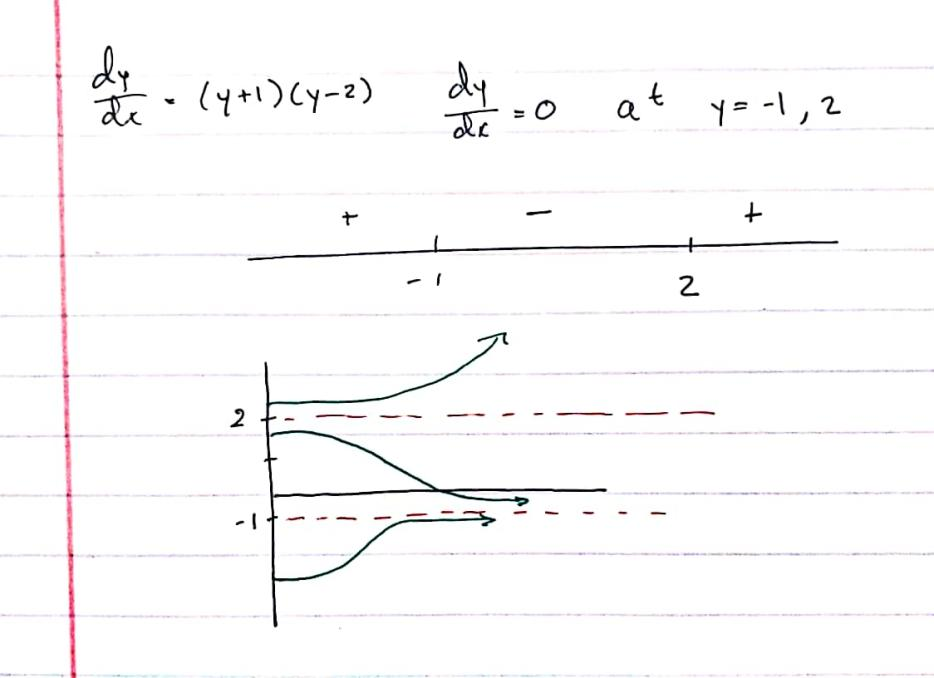
\includegraphics[scale = .3]{number4.jpg}\\
From our equation $\frac{dy}{dx} = (y+1)(y-2)$ we find that the derivative of $y$
is equal to zero when $y = -1, 2$. From there, we can use the snake method to 
see if the derivative is positive or negative when $y < -1, -1<y<2$ and $y > 2$. 
After finding whether the derivative is positive or negative within these respective
intervals, we can draw approximate solutions. 

\item Consider the following initial value problem again:

$\frac{dP}{dt}=0.24P(11-P), P(0)=3$ where $P$ is measured in 100's.

\begin{enumerate}[a)]
\item Why is this a differential equation?\\
\emph{Solution.} \\
This equation has a derivative, which is what makes this an ordinary differential equation. 

\item Use Python to graph $\frac{dP}{dt}$ vs $P$. Include your .py file and  paste your code and your graph below.\\
\emph{Solution.}\\
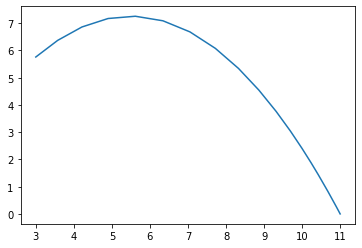
\includegraphics{number5bgraph.png}\\
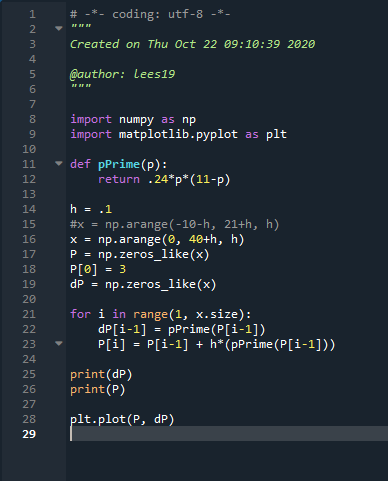
\includegraphics{number5bcode.png}

\item Using your answer to the graph above identify which value(s) of $P$ yield  $\frac{dP}{dt}=0$. Verify that your value(s) of $P$ that you obtained from the graph area also the value(s) of $P$ which algebraically yield $\frac{dP}{dt}=0$.  These are called equilibrium solutions or values or sometimes they are called rest points.
\\
\emph{Solution.}\\
Using the graph above, we see that there is one equlibrium value at $P = 11$. 
This makes sense, as if we plug in $11$ into our $\frac{dP}{dt}$, we find that 
our derivative equals zero, meaning when $P=11$, there is no longer a change in P.
There is also another equlibrium point when $P=0$ which we can find algebraically,
however, we never reach this point on the graph. 

\item How do equilibrium solutions for a differential equation compare to equilibrium solutions of difference equations?  Explain each.
With equilibrium solutions for a differential equation, we are trying to find where the 
derivative is zero. This makes sense, since if the derivative is zero, it means the 
change in the dependent variable is zero, meaning there is no change. With difference equations, 
however, we are finding where the next iteration of the difference equation is the same
as the previous. 

\item Describe the stability of each rest point. Justify your work with graphs and clear mathematical explanations. Your graphs for this part can be hand drawn and pasted in as an image using the {\tt includegraphics} command.\\
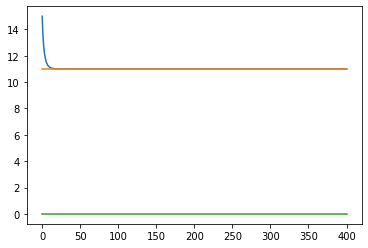
\includegraphics{number5egreater.png}\\
From this graph where the initial value of P is greater than $11$, we find when the 
initial value is greater than $11$, $P$ will still converge back down to $11$. When the 
initial value is between $11$ and $0$, we find that $P$ still converges to $11$. Therefore, 
we can conclude $11$ is a stable equilibrium point. 

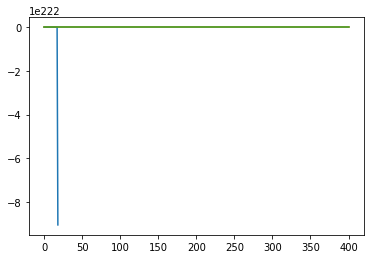
\includegraphics{number5eless.png}
Here we see if the initial value of $P$ is below $0$, it will blow up to negative infinity. 
Therefore, $0$ is not a stable equilibrium value. 

\item For which $P$ value is $\frac{dP}{dt}$ the largest?  What does this mean in terms of the model if this is a model about a disease or rumor spread?
\\
\emph{Solution.}\\
$\frac{dP}{dt}$ seems to be the largest when $P$ is further away from a stable equilibrium point
and then slows down as it gets closer to an equilibrium point. This seems to be 
a model about disease spread. 

\item In terms of this being a rumor spread or disease  spread model, why do your explanations for stability of the equilibrium point(s) make sense?
Zero as an equilibrium point makes sense as if nobody is infected, there is no one to 
spread the disease so the amount of infected will not change. As for $11$ as an equilibrium 
point, if there is a small amount of infected people, that means there will be a large 
amount of susceptible people, which will result in a fast increase in infected people
until it hits an equilibrium value. Starting above the equilibrium value, many people 
are going to be infected, meaning more people are going to be removed, until, again, 
we reach an equilibrium value. 
\end{enumerate}

\item Another method (besides Euler's Method) that is used to solve $y^{\prime}=g(t,y), y(0)=y_0$ is the following:  

Let 

\begin{eqnarray*}
y_{n+1}&=&y_n+\frac{K_1+2K_2+2K_3+K_4}{6}, \mbox{where} \\
K_1&=&g(t_n,y_n)h\\
K_2&=&g(t_n+h/2,y_n+K_1/2)h\\
K_3&=&g(t_n+h/2,y_n+K_2/2)h\\
K_4&=&g(t_n+h,y_n+K_3)h
\end{eqnarray*}
Use this method with a step size of  $h=0.1$ to approximate the solution for the initial value problem in \#5.   Also say the value of $P(2)$  Also obtain  a  plot of the solution over $t \in [0,8]$ . Include your code here and in your compressed folder.
\\
\emph{Solution.} \\
The value for $P(2)$: 
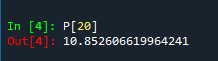
\includegraphics{p2.png}\\

The graph using our new approximation algorithm: \\
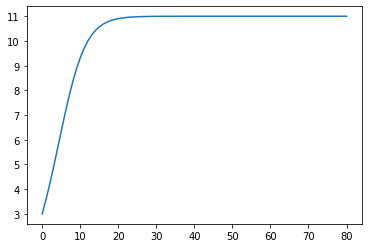
\includegraphics{number6graph.png}\\

Code: \\
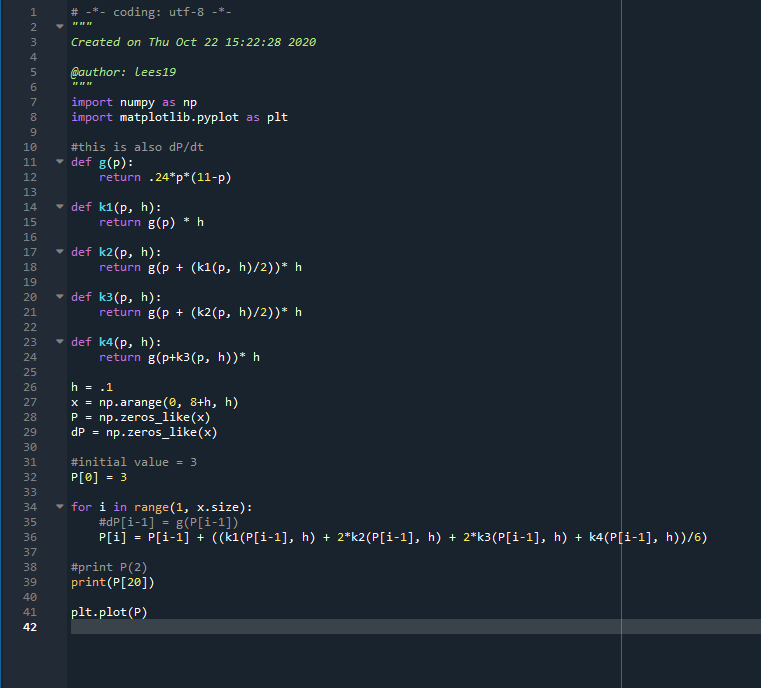
\includegraphics{number6code.png}

\end{enumerate}
\end{document}